\documentclass[xcolor={x11names,svgnames}]{beamer}
\setbeamerfont{note page}{size=\tiny} % default = small 

%\includeonlyframes{radix,radix_code,radix_noconflict}
%\includeonlyframes{lock-free-defs,seq_intset,lf_intset}


\usecolortheme{rose}
\setbeamertemplate{footline}{}
\setbeamertemplate{navigation symbols}{\footnotesize\insertframenumber}
  
\usepackage{amsmath, amssymb, amsthm}

\usepackage[utf8]{inputenc}
\usepackage[francais]{babel}
\usepackage[T1]{fontenc}
\usepackage[normalem]{ulem}   
\usepackage{mdframed}
\usepackage{cancel}

\usepackage{minted}
\setminted{fontsize=\scriptsize}

\usepackage{tikz}
\usetikzlibrary{calc}
\usetikzlibrary{decorations}
\usetikzlibrary{positioning}
\usetikzlibrary{decorations.pathmorphing}
\usetikzlibrary{decorations.pathreplacing}
\usetikzlibrary{shapes.multipart}

\usepackage{fontspec}

\setsansfont{PalatinoSansLTPro}[
   Path = /home/charles/charles_work/fonts/PalatinoSans/, 
   Extension      = .otf,
   UprightFont    = *-Regular,
   BoldFont= *-Bold ,
   ItalicFont = *-Italic,
   BoldItalicFont = *-BoldIta
]

\newcommand{\blue}[1]{{\color{Blue}#1}}
\newcommand{\green}[1]{{\color{LimeGreen}#1}}
\newcommand{\red}[1]{{\color{red}#1}}
\newcommand{\tikzmat}[2] {
\draw[thick] let \p1 = (#1 |- #2),
                 \p2 = (#2 |- #1) in
   ($ (#1) + (0.05,-0.1) $) -- ++(-0.15, 0)  -- ($ (\p1) + (-0.1,0.1) $) -- ++(0.15,0)
   ($ (\p2) + (-0.05,-0.1) $) -- ++(0.15, 0) -- ($ (#2) + (0.1,0.1) $) -- ++(-0.15,0);
}


\author[C.~Bouillaguet]{Charles Bouillaguet \newline
  {\small \texttt{charles.bouillaguet@lip6.fr}}}

\title{Cours 6 : Théorie et pratique \og avancées\fg{} pour la programmation multi-threads}
\date{2020-02-28}


\definecolor{red}{rgb}{1, 0, 0}
\definecolor{Green}{rgb}{0, 0.6, 0}
\definecolor{Purple}{rgb}{0.75, 0, 0.25}

%\newcommand{\red}{\color{red}}
\newcommand{\po}{\xrightarrow{po}}
\newcommand{\net}{\xrightarrow{net}}
\newcommand{\hb}{{\color{blue}\xrightarrow{\texttt{hb}}}}
\newcommand{\rf}{{\color{Green}\xrightarrow{\texttt{rf}}}}
\newcommand{\mo}{{\color{orange}\xrightarrow{\texttt{mo}}}}
\newcommand{\rb}{{\color{Purple}\xrightarrow{\texttt{rb}}}}
\newcommand{\rmw}{{\color{gray}\xrightarrow{\texttt{rmw}}}}
\newcommand{\eco}{{\color{red}\xrightarrow{\texttt{eco}}}}


\begin{document}

\frame{\titlepage}

\begin{frame}[fragile]
  \frametitle{Quizz}

  Initialement, $x = y = 0$.

  \begin{center}
  \begin{tikzpicture}[>=latex,yscale=0.7]
    \path[use as bounding box] (-1, -2) rectangle (7, 4);
    \node<1-2> at (0, 2) (Rx0) {$R_0(x) 0$};
    \node<3> at (0, 4) (Rx0) {$R_0(x) 0$};

    \node<1-2> at (0, 0) (Ry0) {$R_0(y) 1$};
    \node<3> at (0, -2) (Ry0) {$R_0(y) 1$};

    \node<1-2> at (3, 2) (Wx) {$W_1(x) 1$};
    \node<3> at (3, 3) (Wx) {$W_1(x) 1$};

    \node<1-2> at (3, 0) (Wy) {$W_1(y) 1$};
    \node<3> at (3, -1) (Wy) {$W_1(y) 1$};
    
    \node at (6, 2) (Rx1) {$R_2(x) 1$};    
    \node at (6, 0) (Ry1) {$R_3(y) 0$};

    \begin{scope}[every node/.style={font={\ttfamily\small}}]
    \draw (Rx0) edge[->] node[right] {po} (Ry0);
    \draw (Rx1) edge[->] node[right] {po} (Ry1);
    \draw (Wx) edge[->] node[right] {po}  (Wy);

    \draw<2->[Green] (Wx) edge[->] node[above] {rf} (Rx1);
    \draw<2->[Green] (Wy) edge[->] node[above] {rf} (Ry0);
    \draw<2->[Purple] (Rx0) edge[->] node[above] {rb} (Wx);
    \draw<2->[Purple] (Ry1) edge[->] node[above] {rb} (Wy);
  \end{scope}
\end{tikzpicture}
\end{center}

  \begin{block}{Possible ?}
  \begin{enumerate}
  \item Non, c'est contradictoire
  \item Non, car ce n'est pas séquentiellement consistant
  \item Oui, sur les ARM et les POWER mais pas sur les x86 (TSO)
  \item<alert@3-> Oui, car c'est séquentiellement consistant
  \end{enumerate}
\end{block}
\end{frame}

%%%%%%%%%%%%%%%%%%%%%%%%%%%%%%%%%%%%%%%%%%%%%%%%%%%%%%%%%%%%%%%%%%%%%%

\begin{frame}[fragile]
  \frametitle{Quizz (plus dur)}

  Initialement, $x = y = 0$.

  \begin{center}
  \begin{tikzpicture}[>=latex,yscale=0.7]
    \path[use as bounding box] (-1, -2) rectangle (7, 4);
    \node at (0, 2) (Ry0) {$R_0(y) 1$};
    \node at (0, 0) (Rx0) {$R_0(x) 0$};
    \node at (3, 2) (Wx) {$W_1(x) 1$};
    \node at (3, 0) (Wy) {$W_1(y) 1$};    
    \node at (6, 2) (Rx1) {$R_2(x) 1$};    
    \node at (6, 0) (Ry1) {$R_3(y) 0$};

    \begin{scope}[every node/.style={font={\ttfamily\small}}]
    \draw (Ry0) edge[->] node[right] {po} (Rx0);
    \draw (Rx1) edge[->] node[right] {po} (Ry1);
    \draw (Wx) edge[->] node[right] {po}  (Wy);

    \draw<2->[Green] (Wx) edge[->] node[above] {rf} (Rx1);
    \draw<2->[Green] (Wy) edge[->] node[above, very near end] {rf} (Ry0);
    \draw<2->[Purple] (Rx0) edge[->] node[above, very near end] {rb} (Wx);
    \draw<2->[Purple] (Ry1) edge[->] node[above] {rb} (Wy);
  \end{scope}
\end{tikzpicture}
\end{center}

  \begin{block}{Possible ?}
  \begin{enumerate}
  \item Non, c'est contradictoire
  \item Non, car ce n'est pas séquentiellement consistant
  \item<alert@3-> Oui, sur les ARM et les POWER mais pas sur les x86 (TSO)
  \item Oui, car c'est séquentiellement consistant
  \end{enumerate}
\end{block}
\end{frame}


%%%%%%%%%%%%%%%%%%%%%%%%%%%%%%%%%%%%%%%%%%%%%%%%%%%%%%%%%%%%%%%%%%%%%%% 

\begin{frame}[label=golden_rule]
%  \frametitle{}

  \begin{center}
    \Huge \bf \alert{Règle d'or de la \\ programmation multithreads}
  \end{center}

  \bigskip
  
  {\Large \textbf{Tous} les accès potentiellement conflictuels${}^*$ aux variables partagées doivent être protégés (\texttt{atomic}, \texttt{critical}, ...).}

  \bigskip

  $*$ au moins l'un d'entre eux est une écriture.  
\end{frame}


%%%%%%%%%%%%%%%%%%%%%%%%%%%%%%%%%%%%%%%%%%%%%%%%%%%%%%%%

\section{Modifier les algos pour éviter les conflits}

%%%%%%%%%%%%%%%%%%%%%%%%%%%%%%%%%

\begin{frame}[label=idea1]
  \frametitle{Idée générale : \textbf{réorganiser}}

  \begin{columns}[c]
    \begin{column}{.1\textwidth}
      \vspace{1mm}
      \includegraphics[width=\textwidth]{triste.png}
    \end{column}
    
    \begin{column}{.9\textwidth}
      \begin{itemize}
      \item Faire un (tout) petit peu de calculs en plus...
      \end{itemize}
    \end{column}
  \end{columns}

  \vspace{1cm}
  
  \begin{columns}[c]
    \begin{column}{.1\textwidth}
      \vspace{3mm}
      
\includegraphics[width=\textwidth]{Content.png}
    \end{column}
    
    \begin{column}{.9\textwidth}
      \begin{itemize}
      \item ... Pour éliminer complètement les conflits
      \end{itemize}
    \end{column}
  \end{columns}  
\end{frame}

%%%%%%%%%%%%%%


\subsection{Bucket Sort}

%%%%%%%%%%%%%%%%%%%%%%%%%%%%%%%%%%
      \pgfmathdeclarerandomlist{MyRandomColors}{{pink}{red}{orange}{yellow}{green}{cyan}{blue}{magenta}{violet}{lightgray}{darkgray}}

      
\begin{frame}[fragile,label=radix]
  \frametitle{Exemple : Bucket Sort}

%int C[256];
%for (int i = 0; i < 256; i++)
%    C[i] = 0;

    \begin{columns}[c]
    \begin{column}{.4\textwidth}

\begin{minted}{C}
// Initialization
for (int i = 0; i < M; i++)
    C[i] = 0;


// Histogram
for (int i = 0; i < N; i++) {
    int bucket = f(A[i]);
    C[bucket]++;
}

// Prefix-sum
int s = 0;
for (int i = 0; i < M; i++) {
    P[i] = s;
    s += C[i];
}

// Dispatch
for (int i = 0; i < N; i++) {
    int bucket = f(A[i]);
    B[P[bucket]] = A[i];
    P[bucket]++;
}
\end{minted}
    \end{column}
    \begin{column}{.6\textwidth}


      \begin{tikzpicture}[scale=0.25, >={To[sep]}]
        \path[red,dotted,use as bounding box] (-1, 0) rectangle +(26, 32);
        
        % état initial aléatoire
        \pgfmathsetseed{57}
        \foreach \i in {0, 1, ..., 31} {
          \pgfmathrandomitem{\RandomColor}{MyRandomColors} 
          \fill[fill=\RandomColor] (0, \i) rectangle +(3, 1);
        }
        \draw[thick] (0, 0) rectangle +(9, 32);
        \draw[thick] (3, 0) -- +(0, 32);
        \foreach \i in {1, ..., 31} {
          \draw (0, \i) -- +(9, 0);
        }
        \foreach \i / \l in {0/3, 1/0, 2/7, 3/1, 4/10, 5/2, 6/5, 7/2, 8/10, 9/5,
          10/2, 11/3, 12/8, 13/7, 14/9, 15/10, 16/3, 17/6, 18/4, 19/6,
          20/10, 21/0, 22/5, 23/3, 24/5, 25/9, 26/5, 27/7, 28/8, 29/9,
          30/8, 31/5} {
%          \node[font=\tiny] at (-1, 31.5-\i) {\i};
          \node[font=\tiny] at (4, 31.5-\i) {\l};
        }
        
        % côté droit : trié
        \begin{scope}[xshift=16cm]
          % situation finale supposée
          \begin{onlyenv}<1-3>
          \fill[fill=pink] (0, 30) rectangle +(3, 2);
          \fill[fill=magenta] (0, 29) rectangle +(3, 1);
          \fill[fill=violet] (0, 26) rectangle +(3, 3);
          \fill[fill=blue] (0, 22) rectangle +(3, 4);
          \fill[fill=cyan] (0, 21) rectangle +(3, 1);
          \fill[fill=green] (0, 15) rectangle +(3, 6);
          \fill[fill=yellow] (0, 13) rectangle +(3, 2);
          \fill[fill=orange] (0, 10) rectangle +(3, 3);
          \fill[fill=red] (0, 7) rectangle +(3, 3);
          \fill[fill=lightgray] (0, 4) rectangle +(3, 3);
          \fill[fill=darkgray] (0, 0) rectangle +(3, 4);
        \end{onlyenv}

        % \begin{onlyenv}<4->
        %     \fill[very nearly transparent, fill=pink] (0, 30) rectangle +(3, 2);
        %     \fill[very nearly transparent, fill=magenta] (0, 29) rectangle +(3, 1);
        %     \fill[very nearly transparent, fill=violet] (0, 26) rectangle +(3, 3);
        %     \fill[very nearly transparent, fill=blue] (0, 22) rectangle +(3, 4);
        %     \fill[very nearly transparent, fill=cyan] (0, 21) rectangle +(3, 1);
        %     \fill[very nearly transparent, fill=green] (0, 15) rectangle +(3, 6);
        %     \fill[very nearly transparent, fill=yellow] (0, 13) rectangle +(3, 2);
        %     \fill[very nearly transparent, fill=orange] (0, 10) rectangle +(3, 3);
        %     \fill[very nearly transparent, fill=red] (0, 7) rectangle +(3, 3);
        %     \fill[very nearly transparent, fill=lightgray] (0, 4) rectangle +(3, 3);
        %     \fill[very nearly transparent, fill=darkgray] (0, 0) rectangle +(3, 4);
        %   \end{onlyenv}

          % items qui arrivent en cours de route
          \fill<5->[fill=blue] (0, 25) rectangle +(3, 1);
          \fill<9->[fill=pink] (0, 31) rectangle +(3, 1);
          \fill<11->[fill=orange] (0, 12) rectangle +(3, 1);
          
          % cadre
          \draw[thick] (0, 0) rectangle +(9, 32);
          \draw[thick] (3, 0) -- +(0, 32);
          \foreach \i in {1, ..., 31} {
            \draw (0, \i) -- +(9, 0);
          }
      \end{scope}

      % taille des buckets
      \begin{onlyenv}<2>
        \draw[<->] (15, 30) -- node[left] {$C[0]$} +(0, 2);
        \draw[<->] (15, 26) -- node[left] {$C[2]$} +(0, 3);
        \draw[<->] (15, 22) -- node[left] {$C[3]$} +(0, 4);
        \draw[<->] (15, 15) -- node[left] {$C[5]$} +(0, 6);
        \draw[<->] (15, 13) -- node[left] {$C[6]$} +(0, 2);
        \draw[<->] (15, 10) -- node[left] {$C[7]$} +(0, 3);
        \draw[<->] (15, 7) -- node[left] {$C[8]$} +(0, 3);
        \draw[<->] (15, 4) -- node[left] {$C[9]$} +(0, 3);
        \draw[<->] (15, 0) -- node[left] {$C[10]$} +(0, 4);
      \end{onlyenv}

      % pointeurs initiaux sur les buckets
      \begin{onlyenv}<3->
        \draw<-8>[->] (15, 31.5) node[left] {$P[0]$} -- (16, 31.5);
        \draw[->] (15, 28.5) node[left] {$P[2]$} -- (16, 28.5);
        \draw<-5>[->] (15, 25.5) node[left] {$P[3]$} -- +(1, 0);
        \draw[->] (15, 20.5) node[left] {$P[5]$} -- (16, 20.5);
        \draw[->] (15, 14.5) node[left] {$P[6]$} -- (16, 14.5);
        \draw<-11>[->] (15, 12.5) node[left] {$P[7]$} -- (16, 12.5);
        \draw[->] (15, 9.5)  node[left] {$P[8]$} -- (16,  9.5);
        \draw[->] (15, 6.5)  node[left] {$P[9]$} -- (16,  6.5);
        \draw[->] (15, 3.5)  node[left] {$P[10]$}-- (16,  3.5);
      \end{onlyenv}
    
      % pointeurs modifiés
      \draw<6->[->] (15, 24.5) node[left] {$P[3]$} -- +(1, 0);
      \draw<9->[->] (15, 30.5) node[left] {$P[0]$} -- +(1, 0);
      \draw<12->[->] (15, 11.5) node[left] {$P[7]$} -- +(1, 0);
      
      % flèches de progression à gauche
      \draw<4-5>[thick,->] (-2, 31.5) -- +(2, 0);
      \draw<7-8>[thick,->] (-2, 30.5) -- +(2, 0);
      \draw<10-11>[thick,->] (-2, 29.5) -- +(2, 0);

      \draw<5>[->] (9, 31.5) -- (10, 30.5) -- (10, 27) -- (14, 27) -- (16, 26);
      \draw<8>[->] (9, 30.5) -- (14, 30.5) -- (16, 31);
      \draw<11>[->] (9, 29.5) -- (10, 29.5) -- (10, 13.5) -- (14, 13.5) -- (16, 13);
      
\end{tikzpicture}
  
      
    \end{column}
  \end{columns}
\end{frame}

%%%%%%%%%%%%%%%%%%%%%%%%%%%%%%%%%%

\begin{frame}[fragile,label=radix_code]
  \frametitle{Exemple : Bucket Sort}
  \framesubtitle{Parallélisation directe naïve}

    \begin{columns}[c]
    \begin{column}{.6\textwidth}

\begin{onlyenv}<1>
\begin{minted}{C}
// Counting

for (int i = 0; i < N; i++) {
    int bucket = f(A[i]);
    C[bucket]++;
}

// Prefix-sum
int s = 0;
for (int i = 0; i < M; i++) {
    P[i] = s;
    s += C[i];
}

// Dispatch

for (int i = 0; i < N; i++) {
    int bucket = f(A[i]);
    int ptr;

    ptr = P[bucket]++;
    B[ptr] = A[i];
}
\end{minted}
\end{onlyenv}
%
\begin{onlyenv}<2>
\begin{minted}{C}
// Counting
#pragma omp parallel for reduction(+:C[0:M])
for (int i = 0; i < N; i++) {
    int bucket = f(A[i]);
    C[bucket]++;
}

// Prefix-sum (sequential)
int s = 0;
for (int i = 0; i < M; i++) {
    P[i] = s;
    s += C[i];
}

// Dispatch
#pragma omp parallel for
for (int i = 0; i < N; i++) {
    int bucket = f(A[i]);
    int ptr;
    #pragma omp atomic capture
    ptr = P[bucket]++;
    B[ptr] = A[i];
}
\end{minted}
\end{onlyenv}

\end{column}

    \begin{column}{.4\textwidth}

      \begin{tikzpicture}[scale=0.25, >={To[sep]}]
        \path[red,dotted,use as bounding box] (-2, 0) rectangle +(11, 32);
        
        % état initial aléatoire
        \pgfmathsetseed{57}
        \foreach \i in {0, 1, ..., 31} {
          \pgfmathrandomitem{\RandomColor}{MyRandomColors} 
          \fill[fill=\RandomColor] (0, \i) rectangle +(3, 1);
        }
        \draw[thick] (0, 0) rectangle +(9, 32);
        \draw[thick] (3, 0) -- +(0, 32);
        \foreach \i in {1, ..., 31} {
          \draw (0, \i) -- +(9, 0);
        }
        \foreach \i / \l in {0/3, 1/0, 2/7, 3/1, 4/10, 5/2, 6/5, 7/2, 8/10, 9/5,
          10/2, 11/3, 12/8, 13/7, 14/9, 15/10, 16/3, 17/6, 18/4, 19/6,
          20/10, 21/0, 22/5, 23/3, 24/5, 25/9, 26/5, 27/7, 28/8, 29/9,
          30/8, 31/5} {
          \node[font=\tiny] at (4, 31.5-\i) {\l};
        }

        \draw[decorate,decoration={brace,mirror}] (-0.5, 31.9) -- node[left] {$T_0$} +(0, -7.8);
        \draw[decorate,decoration={brace,mirror}] (-0.5, 23.9) -- node[left] {$T_1$} +(0, -7.8);
        \draw[decorate,decoration={brace,mirror}] (-0.5, 15.9) -- node[left] {$T_2$} +(0, -7.8);
        \draw[decorate,decoration={brace,mirror}] (-0.5, 7.9) -- node[left] {$T_3$} +(0, -7.8);
      \end{tikzpicture}
    \end{column}
  \end{columns}
\end{frame}



%%%%%%%%%%%%%%%%%%%%%%%%%%%%%%%%%%

\begin{frame}[label=radix_noconflict]
  \frametitle{Exemple : Bucket Sort}

      \begin{tikzpicture}[scale=0.25, >={To[sep]}]
        \path[red,dotted,use as bounding box] (-1, 0) rectangle +(26, 32);
        
        % état initial aléatoire
        \pgfmathsetseed{57}
        \foreach \i in {0, 1, ..., 31} {
          \pgfmathrandomitem{\RandomColor}{MyRandomColors} 
          \fill[fill=\RandomColor] (0, \i) rectangle +(3, 1);
        }
        \draw[thick] (0, 0) rectangle +(9, 32);
        \draw[thick] (3, 0) -- +(0, 32);
        \foreach \i in {1, ..., 31} {
          \draw (0, \i) -- +(9, 0);
        }
        \foreach \i / \l in {0/3, 1/0, 2/7, 3/1, 4/10, 5/2, 6/5, 7/2, 8/10, 9/5,
          10/2, 11/3, 12/8, 13/7, 14/9, 15/10, 16/3, 17/6, 18/4, 19/6,
          20/10, 21/0, 22/5, 23/3, 24/5, 25/9, 26/5, 27/7, 28/8, 29/9,
          30/8, 31/5} {
          \node[font=\tiny] at (4, 31.5-\i) {\l};
        }
        % threads
        \draw[decorate,decoration={brace,mirror}] (-0.5, 31.9) -- node[left] {$T_0$} +(0, -7.8);
        \draw[decorate,decoration={brace,mirror}] (-0.5, 23.9) -- node[left] {$T_1$} +(0, -7.8);
        \draw[decorate,decoration={brace,mirror}] (-0.5, 15.9) -- node[left] {$T_2$} +(0, -7.8);
        \draw[decorate,decoration={brace,mirror}] (-0.5, 7.9) -- node[left] {$T_3$} +(0, -7.8);

        % côté droit : zoom sur un bucket
        \begin{scope}[xshift=28cm]
        \begin{onlyenv}<1-2>
          \fill[fill=cyan] (0, 26) rectangle +(3, 6);
          \fill[fill=green] (0, 5) rectangle +(3, 21);
          \fill[fill=yellow] (0, 0) rectangle +(3, 5);

          \draw[thick,dotted] (0, 0) -- +(0, 2);
          \draw[thick,dotted] (0, 30) -- +(0, 2);
          \draw[thick,dotted] (3, 0) -- +(0, 2);
          \draw[thick,dotted] (3, 30) -- +(0, 2);
          \draw[thick,dotted] (9, 0) -- +(0, 2);
          \draw[thick,dotted] (9, 30) -- +(0, 2);
          
          \draw[thick] (0, 2) -- +(0, 28);
          \draw[thick] (9, 2) -- +(0, 28);
          \draw[thick] (3, 2) -- +(0, 28);

          \draw[decorate,decoration={brace,mirror}] (-0.5, 25.9) -- node[left] {$T_0$} +(0, -5.8);
          \draw[decorate,decoration={brace,mirror}] (-0.5, 19.9) -- node[left] {$T_1$} +(0, -2.8);
          \draw[decorate,decoration={brace,mirror}] (-0.5, 16.9) -- node[left] {$T_2$} +(0, -6.8);
          \draw[decorate,decoration={brace,mirror}] (-0.5, 9.9) -- node[left] {$T_3$} +(0, -4.8);

          \draw<2>[->] (-5, 25.5) node[left] {$P_0[5]$} -- +(5, 0);
          \draw<2>[->] (-5, 19.5) node[left] {$P_1[5]$} -- +(5, 0);
          \draw<2>[->] (-5, 16.5) node[left] {$P_2[5]$} -- +(5, 0);
          \draw<2>[->] (-5, 9.5) node[left] {$P_3[5]$} -- +(5, 0);

          \foreach \i in {1, ..., 31} {
            \draw (0, \i) -- +(9, 0);
          }
        \end{onlyenv}
      \end{scope}
      
        
        % côté droit : trié                  
        \begin{scope}[xshift=28cm]
        \begin{onlyenv}<3>
          \fill[fill=pink] (0, 30) rectangle +(3, 2);
          \fill[fill=magenta] (0, 29) rectangle +(3, 1);
          \fill[fill=violet] (0, 26) rectangle +(3, 3);
          \fill[fill=blue] (0, 22) rectangle +(3, 4);
          \fill[fill=cyan] (0, 21) rectangle +(3, 1);
          \fill[fill=green] (0, 15) rectangle +(3, 6);
          \fill[fill=yellow] (0, 13) rectangle +(3, 2);
          \fill[fill=orange] (0, 10) rectangle +(3, 3);
          \fill[fill=red] (0, 7) rectangle +(3, 3);
          \fill[fill=lightgray] (0, 4) rectangle +(3, 3);
          \fill[fill=darkgray] (0, 0) rectangle +(3, 4);

          \draw[thick] (0, 0) rectangle +(9, 32);
          \draw[thick] (3, 0) -- +(0, 32);
          \foreach \i in {1, ..., 31} {
            \draw (0, \i) -- +(9, 0);
          }

          % pointeurs initiaux sur les buckets
          \draw[->] (-1, 28.5) node[left] {$P_0[2]$} -- +(1, 0);
          \draw[->] (-7, 26.5) node[left] {$P_1[2]$} -- +(7, 0);
          
          \draw[->] (-1, 20.5) node[left] {$P_0[5]$} -- +(1, 0);
          \draw[->] (-7, 19.5) node[left] {$P_1[5]$} -- +(7, 0);
          \draw[->] (-1, 18.5) node[left] {$P_2[5]$} -- +(1, 0);
          \draw[->] (-7, 17.5) node[left] {$P_3[5]$} -- +(7, 0);
          
          \draw[->] (-1, 9.5) node[left] {$P_1[8]$} -- +(1, 0);
          \draw[->] (-7, 8.5) node[left] {$P_3[8]$} -- +(7, 0);
          
          \draw[->] (-1, 3.5) node[left] {$P_0[10]$} -- +(1, 0);
          \draw[->] (-7, 2.5) node[left] {$P_1[10]$} -- +(7, 0);
          \draw[->] (-1, 0.5) node[left] {$P_2[10]$} -- +(1, 0);
        \end{onlyenv}
      \end{scope}
    \end{tikzpicture}  
\end{frame}

%%%%%%%%%%%%%%%%%%%%%%%%%%%%%%%%%%%

%%%%%%%%%%%%%%%%%%%%%%%%%%%%%%%%%%

\begin{frame}[label=radix_noconflict_table]
  \frametitle{Exemple : Bucket Sort}

      \begin{tikzpicture}[scale=0.25, >={To[sep]}]
        \path[red,dotted,use as bounding box] (-1, 0) rectangle +(26, 32);
        
        % état initial aléatoire
        \pgfmathsetseed{57}
        \foreach \i in {0, 1, ..., 31} {
          \pgfmathrandomitem{\RandomColor}{MyRandomColors} 
          \fill[fill=\RandomColor] (0, \i) rectangle +(3, 1);
        }
        \draw[thick] (0, 0) rectangle +(9, 32);
        \draw[thick] (3, 0) -- +(0, 32);
        \foreach \i in {1, ..., 31} {
          \draw (0, \i) -- +(9, 0);
        }
        \foreach \i / \l in {0/3, 1/0, 2/7, 3/1, 4/10, 5/2, 6/5, 7/2, 8/10, 9/5,
          10/2, 11/3, 12/8, 13/7, 14/9, 15/10, 16/3, 17/6, 18/4, 19/6,
          20/10, 21/0, 22/5, 23/3, 24/5, 25/9, 26/5, 27/7, 28/8, 29/9,
          30/8, 31/5} {
          \node[font=\tiny] at (4, 31.5-\i) {\l};
        }
        % threads
        \draw[decorate,decoration={brace,mirror}] (-0.5, 31.9) -- node[left] {$T_0$} +(0, -7.8);
        \draw[decorate,decoration={brace,mirror}] (-0.5, 23.9) -- node[left] {$T_1$} +(0, -7.8);
        \draw[decorate,decoration={brace,mirror}] (-0.5, 15.9) -- node[left] {$T_2$} +(0, -7.8);
        \draw[decorate,decoration={brace,mirror}] (-0.5, 7.9) -- node[left] {$T_3$} +(0, -7.8);

        \begin{scope}[xshift=13.5cm, yshift=10cm]
          % légendes
          \node[anchor=north east] at (3, 18.75) {$C_i[x] =$};
          \node<1-3>[anchor=north west,align=left] at (3, 19) {\#Élements de catégorie $x$ \\ vus par le thread $i$};
          \node<4-7>[anchor=north west,align=left] at (3, 19) {\#Élements de catégorie $x$ \\ vus par les threads $< i$};
          \node<8->[anchor=north west,align=left] at (3, 18.8) {Indice du début du bucket $x$ \\ pour le threads $i$};
          
          % légende en bas
          \node<2-4>[align=center] at (12, -6) {Taille de chaque bucket};
          \node<6->[align=center] at (12, -6) {Indice du début de chaque bucket\\(\#Élements dans les buckets précédents)};
          
          \foreach \i in {0, 1, 2, 3} {
            \draw[thick] (0, 2*\i) -- +(24, 0);
            \node at (1, 6-2*\i + 1) {\i};
          }
          \draw[<->] (-1, 0) -- node[above, sloped] {Threads} +(0, 8);
          \draw[<->] (2, 11) -- node[above] {Buckets} +(22, 0);
          \draw[ultra thick] (0, 0) -- +(24, 0);
          \draw[ultra thick] (0, 8) -- +(24, 0);
          \node[font=\small] at (1, 9) {$C$};
          \foreach \i in {0, 1, ..., 10} {
            \draw[thick] (2+2*\i, -2) -- +(0, 12);
            \node[font=\small] at (3+2*\i, 9) {\i};
          }
          \draw[ultra thick] (2, -2) -- +(0, 12);

          % compteurs
          \begin{onlyenv}<1-2>
            \foreach \i / \c in {0/1, 1/1, 2/2, 3/1, 5/1, 7/1, 10/1} {
              \node[font=\small] at (3+2*\i, 7) {\c};
            }
            \foreach \i / \c in {2/1, 3/1, 5/1, 7/1, 8/1, 9/1, 10/2} {
              \node[font=\small] at (3+2*\i, 5) {\c};
            }
            \foreach \i / \c in {0/1, 3/2, 4/1, 5/1, 6/2, 10/1} {
              \node[font=\small] at (3+2*\i, 3) {\c};
            }
            \foreach \i / \c in {5/3, 7/1, 8/2, 9/2} {
              \node[font=\small] at (3+2*\i, 1) {\c};
            }
          \end{onlyenv}
          % compteurs prefix-summés
          \begin{onlyenv}<4-7>
            \path (3, 7) foreach \c in {0, ..., 10} { node[font=\small] {0} ++(2, 0) };
            \path (3, 5) foreach \c in {1,1,2,1,0,1,0,1,0,0,1} { node[font=\small] {\c} ++(2, 0) };
            \path (3, 3) foreach \c in {1,1,3,2,0,1,0,2,1,1,3} { node[font=\small] {\c} ++(2, 0) };
            \path (3, 1) foreach \c in {2,1,3,4,1,3,2,2,1,1,4} { node[font=\small] {\c} ++(2, 0) };
          \end{onlyenv}
          % pointeurs vers les débuts des buckets
          \begin{onlyenv}<8->
            \path (3, 7) foreach \c in {0,2,3, 6,10,11,17,19,22,25,28} { node[font=\small] {\c} ++(2, 0) };
            \path (3, 5) foreach \c in {1,3,5, 7,10,12,17,20,22,25,29} { node[font=\small] {\c} ++(2, 0) };
            \path (3, 3) foreach \c in {1,3,6, 8,10,12,17,21,23,26,31} { node[font=\small] {\c} ++(2, 0) };
            \path (3, 1) foreach \c in {2,3,6,10,11,14,19,21,23,26,32} { node[font=\small] {\c} ++(2, 0) };
          \end{onlyenv}

          
          % sommes
          \path<2-5> (3, -1) foreach \c in {2,1,3,4,1,6,2,3,3,3,4} { node[font=\small] {\c} ++(2, 0) };
          \path<6-> (3, -1) foreach \c in   {0,2,3,6,10,11,17,19,22,25,28} { node[font=\small] {\c} ++(2, 0) };
          
          \foreach \i in {0, 1, ..., 10} {
            \draw<2>[very thick,->,red] (3+2*\i, 8) -- +(0, -8.5);
            \draw<3>[very thick,decorate,decoration={snake},->,red] (3+2*\i, 8) -- +(0, -8.5);
            \draw<7>[very thick,->,red] (3+2*\i, -1) -- +(0, 9.2);
          }
          \node<3,5>[red] at (28, 4) {Prefix-Sum};
          \node<2,7>[red] at (28, 4) {Somme};

          % prefix-sum finale sur les tailles de buckets
          \draw<5>[very thick,decorate,decoration={snake},->,red] (2, -1) -- +(21.75, -0);
          
      \end{scope}
    \end{tikzpicture}  
  \end{frame}

%%%%%%%%%%%%%%

\begin{frame}[label=radix_code, fragile]
  \frametitle{Exemple : Bucket Sort}

  \begin{columns}
    \begin{column}{0.5\textwidth}
\begin{minted}{C}
int C[T][M], S[M];

#pragma omp parallel
{
  int t = omp_get_thread_num();

  // Counting
  for (int i = 0; i < M; i++)
      C[t][i] = 0;
  #pragma omp for schedule(static)
  for (int i = 0; i < N; i++) {
      int bucket = f(A[i);
      C[t][bucket]++;
  }
   
  // <<COMPUTE POINTERS>> ------------>

  // Dispatch
  #pragma omp for schedule(static)
  for (int i = 0; i < N; i++) {
      int bucket = f(A[i]);
      int ptr = C[t][bucket]++;
      B[ptr] = A[i];
  }
}
\end{minted}
    \end{column}  

    \begin{column}{5.8cm}
      \vspace{-0.7cm}
%      \begin{mdframed}
      \begin{minted}[frame=single,framesep=3pt]{C}
// sum (columns)
#pragma omp for
for (int i = 0; i < M; i++) {
    S[i] = 0;
    for (int j = 0; j < T; j++)
            S[i] += C[j][i];
}

// horizontal prefix-sum (sequential)
#pragma omp single
{   int s = 0;
    for (int i = 0; i < M; i++) {
        int t = S[i];
        S[i] = s;
        s += t;
}   }

// prefix-sum (columns)
#pragma omp for
for (int i = 0; i < M; i++) {
    int s = S[i];
    for (int j = 0; j < T; j++) {
        int t = C[j][i];
            C[j][i] = s;
            s += t;
}   }
\end{minted}
%      \end{mdframed}
    \end{column}
  \end{columns}
\end{frame}

  
%%%%%%%%%%%%%%%
  
\begin{frame}[label=radix_curve]
  \frametitle{Exemple : Bucket Sort}

  \begin{tikzpicture}
    \node at (0, 0) {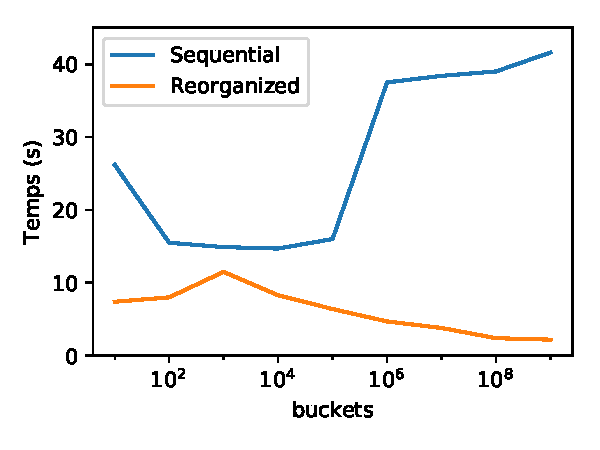
\includegraphics[width=\textwidth]{bucket.pdf}};
    \node at (0, 4) {$N = 10^{10}$};

    \draw[ultra thick,red,->] (-3, -3.75) node[red,left]{$\times 19$}  -| (4.45, -2.1);
  \end{tikzpicture}
\end{frame}

%%%%%%%%%%%%

\begin{frame}[label=radix_code]
  \frametitle{Un tableau d'entiers à trier ?}
  
    \begin{center}
      \Huge \bf \alert{Pro Tip}
  \end{center}

  \begin{exampleblock}{Algorithme de tri parallèle efficace}
    \begin{itemize}
  \item \emph{Parallel Bucket Sort} sur les 8 bits de poids forts
  \item Pour $0 \leq i < 2^8$, faire (en parallèle) :
    \begin{itemize}
    \item Trier le $i$-ème Bucket (avec un tri séquentiel normal)
    \end{itemize}
  \end{itemize}
\end{exampleblock}
  
\end{frame}

%%%%%%%%%%%%%%%%%%%%%%%%%%%%%%%%%%%%%%%%%%%%%%%%%%%%%%%%%%%%%%%%%%%%%%%%%%%%%%%%%%%%%


%%%%%%%%%%%%%%%%%

\section{Tricks transactionnels}

\begin{frame}[label=transactions]
  \frametitle{Transactions parallèles}

  \textbf{lecture} $A[i_1], A[i_2], \dots$ $\rightarrow$ \textbf{calcul} $\rightarrow$ \textbf{écriture} $A[k_1], A[k_2], \dots$.

  \medskip

  \begin{block}{Obstacle à l'exécution \og atomique\fg{} :}
    \begin{itemize}
    \item Les données lues ont été modifiées avant l'écriture.
    \item Résultat du calcul \og périmé\fg{}.
    \end{itemize}
  \end{block}
  
  \begin{overlayarea}{\textwidth}{4cm}
  \begin{alertblock}<only@1>{\textbf{Approche pessimiste} (\og \textit{Ask for Permission}\fg{})}
    \begin{itemize}
    \item \og Verrouiller\fg{} les données lues.
    \item Lecture/Verrouillage $\rightarrow$ Calcul $\rightarrow$ écriture $\rightarrow$ déverrouillage
      \begin{itemize}
      \item Bloque modification \textbf{potentielle} par un autre thread.
      \end{itemize}
    \item Faire comme si le conflit \textbf{ALLAIT} avoir lieu.
    \item Surcoût inutile en l'absence de conflit.
    \end{itemize}
  \end{alertblock}

  \begin{exampleblock}<only@2>{\textbf{Approche optimiste} (\og \textit{Shoot First, Ask Questions Later}\fg{})}
    \begin{itemize}
    \item Lire (\alert{sans précaution !!!}) $\rightarrow$ Calcul $\rightarrow$ \textbf{Commit} (atomique) :
      \begin{itemize}
      \item Vérifier la fraîcheur des données lues,
      \item Si OK, effectuer l'écriture ; sinon, tout recommencer.
      \end{itemize}
    \item Faire comme si le conflit \textbf{N'ALLAIT PAS} avoir lieu.
    \item Travail perdu en cas de conflit.
    \end{itemize}
  \end{exampleblock}    
\end{overlayarea}
\end{frame}

% technique de versioning : couplages sans cycles alternants
%%%%%%%%%%%%%%%%%%%%%%%%%%%%%%%%%%%%%%%%%%%%%%

\begin{frame}[label=idea1]
  \frametitle{Idée générale : \textbf{analyser la fréquence des conflits}}

  \begin{columns}[c]
    \begin{column}{.1\textwidth}
      \vspace{1mm}
      \includegraphics[width=\textwidth]{triste.png}
    \end{column}
    
    \begin{column}{.9\textwidth}
      \begin{itemize}
      \item Prendre le risque de gâcher un peu de calcul...
      \end{itemize}
    \end{column}
  \end{columns}

  \vspace{1cm}
  
  \begin{columns}[c]
    \begin{column}{.1\textwidth}
      \vspace{3mm}
      
\includegraphics[width=\textwidth]{Content.png}
    \end{column}
    
    \begin{column}{.9\textwidth}
      \begin{itemize}
      \item ... Pour réduire le coût de la gestion des conflits
      \end{itemize}
    \end{column}
  \end{columns}  
\end{frame}

%%%%%%%%%%%%%%%%%%%%%%%%%%%%%%%%%%%%%%%%%%%%%%

\begin{frame}[label=versioning]
  \frametitle{Technique générale : le \emph{versioning}}

  \begin{itemize}
  \item Structure de donnée partagée, avec un \alert{numéro de version}
  \item $v = 0$ au début (\alert{impair} pendant les écritures).
  \end{itemize}

  \begin{alertblock}{Écrivain}
    \begin{enumerate}
    \item Entrer section critique ; incrémenter $v$
    \item Effectuer les écritures
    \item incrémenter $v$ ; sortir section critique.
    \end{enumerate}
  \end{alertblock}

  \begin{exampleblock}{Lecteur}
    \begin{enumerate}
    \item $v_{before} \gets v$
    \item Effectuer lectures
    \item $v_{after} \gets v$
    \item Si $v_{before}$ impair ou $v_{before} \neq v_{after}$, recommencer.
    \end{enumerate}
  \end{exampleblock}  
\end{frame}

%%%%%%%%%%%%%%%%%% 

\begin{frame}
    \frametitle{Technique générale : le \emph{versioning}}

    \begin{center}
      \begin{tikzpicture}[scale=0.9, every node/.style={font=\small}]
        \foreach \i in {0, 1, 2, 3} {
          \node at (-0.5, 0.5 + \i)  {$T_\i$};
        }
        \node at (-0.5, -0.5)  {$T_w$};
        \draw[dashed] (3, -1.5) -- +(0, 5.75);
        \draw[dashed] (8, -1.5) -- +(0, 5.75);
        
  % lectures avant
  \draw[fill=white] (0.5, 1) rectangle node {reads} +(1, 0.75);
  \draw[fill=white] (0.75, 3) rectangle node {reads} +(1, 0.75);  
  
  % lecture échouent 
  \draw[fill=gray] (2, 0) rectangle node {reads} +(4, 0.75);
  \draw[fill=gray] (2.5, 1) rectangle node {reads} +(5, 0.75);
  \draw[fill=gray] (1, 2) rectangle node {reads} +(3, 0.75);
  \draw[fill=gray] (2.5, 3) rectangle node {reads} +(2, 0.75);
  \draw[fill=gray] (7, 0) rectangle node {reads} +(2, 0.75);
  \draw[fill=gray] (5, 2) rectangle node {reads} +(1, 0.75);
  \draw[fill=gray] (7, 2) rectangle node {reads} +(3, 0.75);
  \draw[fill=gray] (5, 3) rectangle node {reads} +(4, 0.75);

  % lectures après
  \draw[fill=white] (9.5, 0) rectangle node {reads} +(1, 0.75);  
  \draw[fill=white] (8.5, 1) rectangle node {reads} +(1, 0.75);
  \draw[fill=white] (10.5, 2) rectangle node {reads} +(1, 0.75);  
  \draw[fill=white] (10, 3) rectangle node {reads} +(1, 0.75);

  % thread écrivain
  \draw[fill=yellow] (3.25, -1) rectangle node[] {write} +(4.5, 0.75);
\end{tikzpicture}
\end{center}

\begin{itemize}
\item Écrivains prioritaires sur les lecteurs
\end{itemize}


\end{frame}

%%%%%%%%%%%%%%%%%%%%%%%%%%%%%%%%%%%%%%%%%%%%%%%

\begin{frame}[label=urmatching]
  \frametitle{Exemple : plus grand couplage sans cycle alternant}

  \begin{center}
  \begin{tikzpicture}[xscale=1.41,>=stealth,yscale=1.2]

\node at (0, 2) (R1) {A};
\node at (0, 1) (R2) {B};
\node at (0, 0) (R3) {C};
\node at (1,2) (C1) {1};
\node at (1,1) (C2) {2};
\node at (1,0) (C3) {3};
\draw[blue] (C1) edge (R2);
\draw[blue] (C2) edge (R1);
\draw(R2)--(C3);
\draw[red,very thick] (R1) edge (C1);
\draw[red,very thick] (R2) edge (C2);
\draw[very thick](R3)--(C3);
\draw (C3) +(-0.5, -0.2) node[align=center,below,font=\footnotesize]{Couplage avec \red{\textbf{c}}\blue{y}\red{\textbf{c}}\blue{l}\red{\textbf{e}} \blue{a}\red{\textbf{l}}\blue{t}\red{\textbf{e}}\blue{r}\red{\textbf{n}}\blue{a}\red{\textbf{n}}\blue{t} \\ (polynomial)};


\begin{scope}[xshift=4cm]
  \node at (0, 2) (RR1) {A};
\node at (0, 1) (RR2) {B};
\node at (0, 0) (RR3) {C};
\node at (1,2) (CC1) {1};
\node at (1,1) (CC2) {2};
\node at (1,0) (CC3) {3};
\draw (CC1) edge (RR2);
\draw (RR1) edge (CC2);
\draw[very thick] (CC1) edge (RR1);
\draw[very thick] (RR2) edge (CC3);
\draw (RR1) edge (CC1);
\draw (RR2) edge (CC2);
\draw (RR3) edge (CC3);
\draw (CC3) +(-0.5, -0.2) node[below,font=\footnotesize,align=center]{Couplage sans cycle alternant \\ (NP-dur)};
\end{scope}
\end{tikzpicture}
\end{center}

\begin{block}{Algorithme glouton \uncover<2>{parallèle avec \textbf{\bfseries Versioning}}}
  Pour tout sommet $u$ (en parallèle) et toute arête $(u \leftrightarrow v)$  :
  \begin{itemize}
  \item<2-> $t \gets |\mathcal{C}|$ 
  \item Parcours en largeur \blue{a}\red{\textbf{l}}\blue{t}\red{\textbf{e}}\blue{r}\red{\textbf{n}}\blue{a}\red{\textbf{n}}\blue{t} depuis $u$ ; atteint $v$ ? $\Rightarrow$ \texttt{abort}.
  \item<only@1> Ajoute $(u \leftrightarrow v)$ à $\mathcal{C}$. \hfill \textit{[OK, pas de cycle]} 
  \item<only@2> \textbf{section critique} : si $t = |\mathcal{C}|$, ajoute $(u \leftrightarrow v)$ à $\mathcal{C}$ ; ok $\gets 1$.
  \item<2> Si $ok = 0$, recommencer.\hfill\textit{[KO, couplage modifié]} 
  \end{itemize}
\end{block}
\end{frame}

%%%%%%%%%%%%%%%%%%%%%%%%%%%%%%

\section{Support Hardware pour la concurrence}

\begin{frame}[fragile, label=rtm]
  \frametitle{Concept de \og transaction \fg{}}

  \begin{itemize}
  \item Problèmes similaires dans les serveurs de bases de données
  \item Nombreuses techniques de gestion des transactions
  \end{itemize}

  \begin{columns}
    \begin{column}{0.47\textwidth}
  \begin{alertblock}{CPU (très) modernes :\\ \textbf{transactional memory}}
\begin{minted}{C}
#include <immintrin.h>
unsigned int status = _xbegin();
if (status == _XBEGIN_STARTED) {
    // Access shared data ...
    if (problem)    // give up ?
        _xabort(0); 
    // Access more shared data ...
    _xend();
    /* <-------- Success !!! */
} else { /* <--- Failure */
    if (status & _XABORT_EXPLICIT)
        ...
    if (status & _XABORT_CONFLICT)
        ...    
    if (status & _XABORT_CAPACITY)
        ...
}
\end{minted}
  \end{alertblock}
\end{column}
\begin{column}{0.63\textwidth}
  \begin{itemize}
  \item \verb|_xbegin()| démarre une transaction
    \begin{itemize}
    \item Renvoie \verb|_XBEGIN_STARTED|
    \item Purge le cache...
    \end{itemize}
  \item \verb|_xend()| tente le \og commit\fg{}.
    \begin{itemize}
    \item OK $\rightarrow$ l'exécution continue.
    \end{itemize}
  \item \verb|_xabort(cst)| force l'échec

    \medskip

  \item \alert{En cas d'échec} :
    \begin{itemize}
    \item Retourne après \verb|_xbegin()|
    \item Code erreur (conflit, resources, ...)
    \end{itemize}

    \medskip

  \item Toujours pas la panacée
    \begin{itemize}
    \item Coût non-négligeable
    \item Faux-positifs, ...
    \end{itemize}

    \medskip

  \item Cf. aussi bibliothèque \texttt{TinySTM}
  \end{itemize}
\end{column}
\end{columns}
\end{frame}

%%%%%%%%%%%%%%%%%%%%%%%%%%%%%%%%%%%%%%%%

\begin{frame}[fragile, label=CAS]
  \frametitle{L'opération \emph{Compare-And-Swap}}

  \small
  \begin{itemize}
  \item OpenMP spécifie un \emph{modèle mémoire} et des \emph{opérations
      atomiques} séquentiellement consistantes.
  \item \textbf{C11} (ISO/IEC 9899:2011) donne des équivalents.
  \item Avec un (gros) bonus : \textbf{\emph{compare-and-swap} \alert{atomique}}.
  \end{itemize}

\medskip
  
\begin{minted}{C}
#include <stdatomic.h>
bool atomic_compare_exchange_strong(volatile A* obj, C* expected, C desired);
bool atomic_compare_exchange_weak(volatile A *obj, C* expected, C desired);
\end{minted}

\medskip

\begin{block}{Spécification --- version \emph{strong}}
  \mintinline{C}{ok = (obj == expected); if (ok) obj = desired; return ok}% \hfill\alert{(atomique !)}
\end{block}

\medskip

\begin{enumerate}
\item Instruction du CPU (ou versions équivalents LL/SC)
\item La version \emph{weak} peut avoir des faux négatifs
\end{enumerate}

\end{frame}

%%%%%%%%%%%%%%%%%%%%%%%%%%

\begin{frame}[fragile]
  \frametitle{Et dans OpenMP ?}

  \begin{columns}[b]
    \begin{column}{.1\textwidth}
      
\includegraphics[width=\textwidth]{Content.png}
    \end{column}
    \begin{column}{.9\textwidth}
      \begin{itemize}
      \item Compare-and-swap est dans OpenMP 5.1
      \item Paru en novembre 2020
      \end{itemize}
    \end{column}
  \end{columns}

\bigskip
  
\begin{minted}[fontsize=\normalsize]{C}
#pragma omp atomic compare
if (obj == expected)
        obj = desired;

#pragma omp atomic compare capture
if (obj == expected)
        obj = desired;
else
        v = obj;
\end{minted} 

\bigskip

\begin{columns}[b]
    \begin{column}{.1\textwidth}
      
\includegraphics[width=\textwidth]{Triste.png}
    \end{column}
    \begin{column}{.9\textwidth}
      \begin{itemize}
      \item \texttt{gcc} 10.2 ne l'implante pas encore...
      \end{itemize}
    \end{column}
  \end{columns}

\end{frame}

%%%%%%%%%%%%%%%%%%%%%%%%%%

\begin{frame}[fragile, label=CAS]
  \frametitle{Transactions avec \emph{Compare-And-Swap}}

  On peut faire (presque) n'importe quoi avec \emph{Compare-And-Swap} !

  \bigskip
  
  \begin{block}{Idée générale : \emph{Compare-And-Swap Loop}}
    \begin{enumerate}
    \item~[Begin.] $x_{old} \gets x$ 
    \item~[Work.] Calculer une mise à jour $x_{new}$
    \item~[Commit.] \mintinline{C}{ok = atomic_compare_exchange_strong(x, x_old, x_new)}
    \item~[Repeat.] Si pas \texttt{ok}, retourner en 1.
      \end{enumerate}
    \end{block}
  \end{frame}
  
\begin{frame}[fragile, label=CAS_list]
  \frametitle{Exemples avec \emph{Compare-And-Swap}}

  \begin{exampleblock}{Exemple : liste chainée}
\begin{minted}{C}
struct item_t {
    ...
    struct item_t *next;
}

void atomic_append(struct item_t *list, ...)
{
    struct item_t *new =  malloc(sizeof(*new));
    ...
    bool ok = false;
    while (!ok) {
        new->next = list;
        ok =  atomic_compare_exchange_strong(list, new->next, new);
    }
}
\end{minted}
    \end{exampleblock}
\end{frame}

%%%%%%%%%%%%%%%%%%%%%%%%

\begin{frame}[fragile, label=CAS_hash]
  \frametitle{Exemples avec \emph{Compare-And-Swap}}

  \begin{exampleblock}{Exemple : table de hachage avec sondage linéaire}
\begin{minted}{C}
void insert(void *H, void *item)
{
    int i = hash_function(item);        // hash
    while (H[i] != EMPTY)               // trouve une case vide
        i = (i + 1) % HASHTABLE_SIZE;        
    H[i] = item;                        // insert
}
\end{minted}
  \end{exampleblock}

\medskip
  
  \begin{alertblock}{Version thread-safe}
\begin{minted}{C}
void ATOMIC_insert(void *H, void *item)
{
    int i = hash_function(item);
    book ok = false
    while (!ok) {
        ok = atomic_compare_exchange_strong(H[i], EMPTY, item);
        i = (i + 1) % HASHTABLE_SIZE;        
    }
}
\end{minted}
  \end{alertblock}
\end{frame}

%%%%%%%%%%%%%%%%%%%%%%%%%%%%%%%%%%%%%%%%%%%%%%%%%%%%%%%%%%

\begin{frame}[label=lock-free-defs]
  \frametitle{Idée générale : algorithmes \emph{lock-free}}

  \begin{block}{Définition}
    Une fonction est \textbf{lock-free} si, lorsqu'elle est appelée par plusieurs
    threads à la fois, au moins l'une des invocations termine en un nombre fini
    d'étapes de calcul (quoi que fassent les autres, même s'ils bloquent).
  \end{block}

  \bigskip
  
  Remarque : si une fonction acquiert un verrou / section critique, elle ne peut
  pas être \emph{lock-free}.

  \pause\bigskip
  
  \begin{tikzpicture}
    \node (switch) {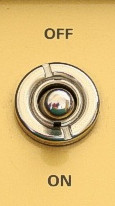
\includegraphics[width=2cm]{switch.jpg}};
    \node[above right=-10mm and 0mm of switch, font={\Large\bfseries}] {Safety};
    \node[below right=-10mm and 0mm of switch, text=red, font={\Large\bfseries}] {World of PAIN};
    \node[left=of switch, font={\large}] (label) {Guru switch};
    \draw (label) edge[->] (switch);
  \end{tikzpicture}

\end{frame}

%%%%%%%%%%%%%%%%%%%%%%%%%%%%%%%%%%%%%%%%%%%%%%%%%%%%%%%%%

\begin{frame}[fragile,label=seq_intset]
  \frametitle{Exemple : ensemble d'entiers}

  \begin{tabular}{c|c}
\begin{minipage}[t]{0.55\textwidth}
\begin{minted}[fontsize=\scriptsize]{C}
bool * A;   
int N, min;  

// A[i] indique si i est dans l'ensemble
// min pointe sur le plus petit élément

void setup()
{
   A = malloc((N + 1) * sizeof(*A));
   // astuce : sentinelle en position N
   for (int i = 0; i < N + 1; i++)
      A[i] = true;
   min = 0;
}
\end{minted}
\end{minipage}
  &
\begin{minipage}[t]{0.45\textwidth}
\begin{minted}[fontsize=\scriptsize]{C}
bool remove(int i)
{
    bool x = A[i];
    A[i] = false;
    return x;
}

int extract_min()
{
   while(A[min] == false)
      min++;
   if (min < N)
      remove(min);
   return min;
}
\end{minted}
\end{minipage}
  \end{tabular}

\begin{alertblock}{Invariants}
  \texttt{A[N] == true} et \texttt{A[0:min] == false}.
\end{alertblock}
\end{frame}

%%%%%%%%%%%%%%%%%%%%%%%%%%%

\begin{frame}[fragile,label=lf_intset]
  \frametitle{Exemple : ensemble d'entiers \alert{lock-free}}
  
\begin{minted}[fontsize=\scriptsize]{C}
#include <stdbool.h>
#include <stdatomic.h>
#define CAS atomic_compare_exchange_weak

_Atomic bool * A;         
_Atomic int min;          
int N;
bool yes = true;

void setup()
{
    A = malloc((N + 1) * sizeof(*A));
    for (int i = 0; i < N + 1; i++)
        atomic_store(&A[i], true);
    atomic_store(&min, 0);
}

bool remove(int i)
{
    return atomic_exchange(&A[i], false);    // comme précédemment
}
\end{minted}
\end{frame}

%%%%%%%%%%%%%%%%%%%%%%%%%%%


\begin{frame}[fragile,label=lf_intset]

  \smallskip
  
\begin{alertblock}{Invariants}
  \texttt{A[N] == true} et \texttt{A[0:min] == false}.
\end{alertblock}

\begin{overlayarea}{\textwidth}{8cm}
\begin{minted}[fontsize=\scriptsize]{C}
int extract_min()
{
    int old_min = atomic_load(&min);
    int i = old_min;               // cherche A[i] == true
    while(atomic_load(&A[i]) == false)
        i++;
\end{minted}
\begin{onlyenv}<2->%
\begin{minted}[fontsize=\scriptsize]{C}
    if (i == N) {                  // ensemble vide ?
        atomic_store(&min, N);     
        return N;
     }
\end{minted}
\end{onlyenv}%
\begin{onlyenv}<3>
\begin{minted}[fontsize=\scriptsize]{C}
    atomic_store(&A[i], false);
  \end{minted}
  \begin{block}{Raté}
    \begin{itemize}
    \item On a bien vu \texttt{A[i] == true} ...
    \item ... mais ça a pu changer entre-temps ...
    \item Si un autre \texttt{extract\_min()} a eu lieu en même temps
    \end{itemize}
  \end{block}
\end{onlyenv}
\begin{onlyenv}<4->
\begin{minted}[fontsize=\scriptsize]{C}
    bool ok = CAS(&A[i], &yes, false);
    if (!ok)         
        return extract_min();      // A[i] == false ? On recommence   
\end{minted}
\end{onlyenv}
\begin{onlyenv}<5>
\begin{minted}[fontsize=\scriptsize]{C}
    CAS(&min, &old_min, i);        // avance min (paresseusement)
    return i;
}
\end{minted}
\end{onlyenv}
\begin{onlyenv}<6->
\begin{minted}[fontsize=\scriptsize]{C}
    while(old_min < i) {           // avance min (consciencieusement)
        bool ok = CAS(&min, &old_min, i);
        if (ok)
            break;
        old_min = atomic_load(&min);
    }
    return i;
}
\end{minted}
\end{onlyenv}
\end{overlayarea}

\end{frame}

%%%%%%%%%%%%%%%%%%%%%%%%%%%%%%%%

\begin{frame}[label=lf_intset]
  \frametitle{La question à 20\ 000 points}

  {\Huge Est-ce correct ?}

  \bigskip\pause

  \begin{alertblock}{Question subsidiaire}
    Que signifie \og être correct\fg{} ?
  \end{alertblock}

  \bigskip\pause
  
  \begin{exampleblock}{Définition}
    Une structure de donnée est \textbf{linéarisable} si tout se passe comme si les
    fonctions qui y accèdent prenaient effet \emph{instantanément}, à un point
    quelconque entre leur invocation et leur terminaison.
  \end{exampleblock}

  \bigskip\pause

  Correct $\approx$ linéarisable

  \bigskip\pause

  Exercice : faites la preuve.
\end{frame}

\end{document}




%%% Local Variables:
%%% TeX-command-extra-options: "-shell-escape"
%%% TeX-engine: xetex
%%% ispell-local-dictionary: "french"
%%% eval: (flyspell-mode 1)
%%% eval: (reftex-mode 1)
%%% End:
